
% ------------------------ Prototype ------------------------

\section*{APPENDIX A - Prototype \label{sec:proto}}
\addcontentsline{toc}{section}{APPENDIX A - Prototype}


\begin{comment}

    Provide the filtered part of RM showing selected features for prototype building. State the detailed steps of compilation, execution and setups. Specify prototype details showing codes, screens, test data, sample output and detailed steps of compilation, execution and setups (if any).

\end{comment}

% ---------- Start the prototype appendix

\begin{tcolorbox}[colback=gray!5!white, colframe=gray!80!black, boxrule=0.5pt, title=Import Libraries and Setup]
    \begin{lstlisting}[language=Python]
    import streamlit as st
    import joblib
    import pandas as pd
    import praw
    from PIL import Image
    from deep_translator import GoogleTranslator
    import requests
    from io import BytesIO
    from collections import Counter
    import google.generativeai as genai
    import pytesseract
    
    pytesseract.pytesseract.tesseract_cmd = '/usr/bin/tesseract'
    \end{lstlisting}
    \end{tcolorbox}
\noindent
This section imports necessary libraries such as streamlit for the web interface, joblib for loading pre-trained models, pandas for data manipulation, praw for interacting with Reddit, and pytesseract for Optical Character Recognition (OCR). It also sets the Tesseract executable path for OCR.    

\begin{tcolorbox}[colback=gray!5!white, colframe=gray!80!black, boxrule=0.5pt, title=Reddit API Setup and Functions]
    \begin{lstlisting}[language=Python]
    # Initialize Reddit API
    reddit = praw.Reddit(client_id='<REDDIT_CLIENT_ID>',
                         client_secret='JREDDIT_CLIENT_SECRET',
                         user_agent='Mental Health')
    
    # Function to fetch text-based posts from Reddit
    def fetch_user_text_posts(username):
        try:
            user = reddit.redditor(username)
            posts = [post.title + " " + post.selftext for post in user.submissions.new(limit=20)]
            return posts
        except Exception as e:
            st.write(f"Error fetching text posts: {e}")
            return []
    \end{lstlisting}
    \end{tcolorbox}
\noindent
This part sets up the Reddit API using praw to interact with Reddit. It also defines a function fetch\_user\_text\_posts that fetches the latest 20 posts from a given Reddit username, returning their title and self-text.

\begin{tcolorbox}[colback=gray!5!white, colframe=gray!80!black, boxrule=0.5pt, title=Image OCR Functionality]
    \begin{lstlisting}[language=Python]
    # Function to fetch image-based posts from Reddit and perform OCR
    def fetch_user_images_and_extract_text(username):
        try:
            user = reddit.redditor(username)
            images = [post.url for post in user.submissions.new(limit=20) if post.url.endswith(('.jpg', '.jpeg', '.png', '.webp', '.bmp', '.tiff'))]
    
            extracted_texts = []
            for image_url in images:
                try:
                    response = requests.get(image_url)
                    image = Image.open(BytesIO(response.content))
                    st.image(image, caption="Fetched Image", use_column_width=True)
    
                    # Extract text from image
                    extracted_text = extract_text_from_image(image)
                    extracted_text = "\n".join(extracted_text)
    
                    # Translate to English if needed
                    if extracted_text.strip():
                        translated_text = GoogleTranslator(source='auto', target='en').translate(extracted_text)
                        extracted_texts.append(translated_text)
                        st.write("Extracted and Translated Text from Image:")
                        st.text(translated_text)
                except Exception as e:
                    st.write(f"Error processing image {image_url}: {e}")
    
            return extracted_texts
        except Exception as e:
            st.write(f"Error fetching images: {e}")
            return []

            # Function to extract text from image using Tesseract
            def extract_text_from_image(image):
                extracted_text = pytesseract.image_to_string(image)
                return extracted_text.splitlines()
    \end{lstlisting}
    \end{tcolorbox}
\noindent
The above code fetches image posts from a Reddit user's submissions and extracts text from those images using OCR (Tesseract). It also translates the extracted text into English if necessary.

\begin{tcolorbox}[colback=gray!5!white, colframe=gray!80!black, boxrule=0.5pt, title=Text Classification and Wellbeing Insight]
    \begin{lstlisting}[language=Python]

    # Configure the Gemini API for wellbeing mapping
    genai.configure(api_key="<GEMINI_API_KEY>")
    generation_config = {
        "temperature": 1,
        "top_p": 0.95,
        "top_k": 40,
        "max_output_tokens": 8192,
        "response_mime_type": "text/plain",
    }
    gemini_model = genai.GenerativeModel(
        model_name="gemini-1.5-flash",
        generation_config=generation_config,
    )

    # Function to classify text and display result
    def classify_text(text):
        input_vectorized = vectorizer.transform([text])
        prediction_proba = model.predict_proba(input_vectorized)
    
        issue_labels = model.classes_
        proba_df = pd.DataFrame(prediction_proba, columns=issue_labels).T
        proba_df.columns = ['Probability']
    
        top_issue = proba_df['Probability'].idxmax()
        top_probability = proba_df['Probability'].max()
    
        st.write(f"The most likely mental health concern is: {top_issue} with a probability of {top_probability:.2%}")
    
        # Call the Gemini model to get well-being insights
        get_wellbeing_insight(text, top_issue)
    \end{lstlisting}
\end{tcolorbox}

\begin{tcolorbox}[colback=gray!5!white, colframe=gray!80!black, boxrule=0.5pt, title=Text Classification and Wellbeing Insight]
    \begin{lstlisting}[language=Python]
    # Function to get well-being insights from Gemini model
    def get_wellbeing_insight(text, top_issue):
        try:
            chat_session = gemini_model.start_chat(history=[])
            prompt = f"Analyze the following text for mental wellbeing insights related to {top_issue}: {text}. Based on this, provide practical advice or actions the user can take to reduce or improve {top_issue}. Be supportive and provide actionable suggestions."
            response = chat_session.send_message(prompt)
    
            st.write("### Wellbeing Insight:")
            st.write(response.text)
        except Exception as e:
            st.write(f"Error retrieving wellbeing insights: {e}")
    \end{lstlisting}
    \end{tcolorbox}
\noindent
The classify\_text function takes text input, vectorizes it using a pre-trained vectorizer, and predicts the most likely mental health issue. It also calls the Gemini model to provide wellbeing insights and advice.    

\begin{tcolorbox}[colback=gray!5!white, colframe=gray!80!black, boxrule=0.5pt, title=Main Streamlit Application Logic]
    \begin{lstlisting}[language=Python]
        # Define the Streamlit app
        def run_app():
            st.title("Mental Health Classifier App")
        
            # Option to choose functionality
            option = st.sidebar.selectbox(
                "Choose an option",
                ["Text Input", "Image Upload", "Reddit Username Analysis"]
            )
        \end{lstlisting}
    \end{tcolorbox}
    \noindent
    There are options to predict only text, predict only image or input a reddit username. The username would be used along with PRAW to extract the top 20 texts and 20 images from the recent posts. This extracted data would then be used further for mental health classification. Also Gemini AI would help in mapping this mental health issue with probable mental wellbeing.

    \begin{tcolorbox}[colback=gray!5!white, colframe=gray!80!black, boxrule=0.5pt, title=Main Streamlit Application Logic]
        \begin{lstlisting}[language=Python]

    # 1. Text Input
    if option == "Text Input":
        st.subheader("Enter Text to Classify Mental Health Issue")
        input_text = st.text_area("Enter your text here:")

        if st.button("Classify Text"):
            if input_text.strip() == "":
                st.write("Please enter some text to classify.")
            else:
                # Translate if not in English
                translated_text = GoogleTranslator(source='auto', target='en').translate(input_text)
                st.write("Translated Text (to English):")
                st.write(translated_text)

                # Classify and display result
                classify_text(translated_text)

    # 2. Image Upload
    elif option == "Image Upload":
        st.subheader("Upload an Image to Extract and Classify Text")
        uploaded_image = st.file_uploader("Upload an Image", type=["jpg", "jpeg", "png", "webp", "bmp", "tiff"])

        if uploaded_image is not None:
            image = Image.open(uploaded_image)
            st.image(image, caption="Uploaded Image", use_column_width=True)

            # Extract text from image
            extracted_text = extract_text_from_image(image)
            extracted_text = "\n".join(extracted_text)

            st.subheader("Extracted Text")
            st.text(extracted_text)
        
            # Translate text to English if needed
            translated_text = GoogleTranslator(source='auto', target='en').translate(extracted_text)
            st.subheader("Translated Text (to English)")
            st.text(translated_text)
        \end{lstlisting}
    \end{tcolorbox}

    \begin{tcolorbox}[colback=gray!5!white, colframe=gray!80!black, boxrule=0.5pt, title=Main Streamlit Application Logic]
        \begin{lstlisting}[language=Python]
        if st.button("Classify Extracted Text"):
            classify_text(translated_text)
        
        # 3. Reddit Username Analysis
        elif option == "Reddit Username Analysis":
            st.subheader("Enter Reddit Username for Analysis")
            username = st.text_input("Enter Reddit username:")
        
            if st.button("Analyze"):
                if username.strip() == "":
                    st.write("Please enter a Reddit username.")
                else:
                    # Fetch and display text posts
                    text_posts = fetch_user_text_posts(username)
                    if text_posts:
                        st.write("Recent Text Posts:")
                        st.write(text_posts[:3])  # Display a few posts for review
        
                    # Fetch and display image-based posts with extracted text
                    image_texts = fetch_user_images_and_extract_text(username)

            # Combine text from both text posts and image text
            all_text = text_posts + image_texts
            if all_text:
                predictions = []
                for text in all_text:
                    # Vectorize and classify each post
                    input_vectorized = vectorizer.transform([text])
                    prediction = model.predict(input_vectorized)
                    predictions.append(prediction[0])
            
            # Count the most common mental health issue
            issue_counts = Counter(predictions)
            top_issue, top_count = issue_counts.most_common(1)[0]
            top_percentage = (top_count / len(predictions)) * 100
                \end{lstlisting}
            \end{tcolorbox}

        \begin{tcolorbox}[colback=gray!5!white, colframe=gray!80!black, boxrule=0.5pt, title=Main Streamlit Application Logic]
            \begin{lstlisting}[language=Python]
            st.write(f"The most frequently detected mental health concern is: {top_issue} appearing in {top_percentage:.2f}% of analyzed text.")
            issue_distribution = pd.DataFrame(issue_counts.items(), columns=['Mental Health Issue', 'Count'])
            st.write("Mental health issue distribution across posts:")
            st.write(issue_distribution)

            # Call the Gemini model to get well-being insights
            get_wellbeing_insight(" ".join(all_text), top_issue)
        else:
            st.write("No valid text found for analysis.")
    
    # Run the app
    if __name__ == '__main__':
        run_app()
    \end{lstlisting}
    \end{tcolorbox}
                
\noindent
This section defines the main structure of the Streamlit app, providing options for users to input text, upload images, or analyze Reddit usernames. Each option triggers different functionalities like text classification, image-based text extraction, and Reddit post analysis.    
\newline
\newline
\noindent
The main logic of the Streamlit application focuses on text and image classification for mental health issues, alongside an analysis of Reddit posts. The application offers three primary features: text input, image upload, and Reddit username analysis. For text input, users can enter text which is automatically translated into English if needed. The translated text is then passed to a classifier, which determines the most probable mental health concern based on the content. If the user uploads an image, the application extracts text from the image using OCR (Optical Character Recognition), translates it to English if necessary, and then classifies the extracted text. The Reddit username analysis feature allows users to input a Reddit username. The application fetches the most recent posts by the user, classifies both text-based and image-based posts, and then aggregates the results to identify the most frequent mental health issue discussed. If both text and image data are available, the application analyzes all content, classifies the posts, and provides insights into the most commonly detected issue. It also visualizes the distribution of detected issues and uses the Gemini AI model to provide well-being advice and actionable steps for users. The code integrates multiple components including the `GoogleTranslator` for text translation, Tesseract for image text extraction, and a pre-trained logistic regression model to classify text data. Additionally, it uses the Gemini API to generate well-being insights based on the classified mental health concerns.

\begin{figure}[h!]  
    \centering
    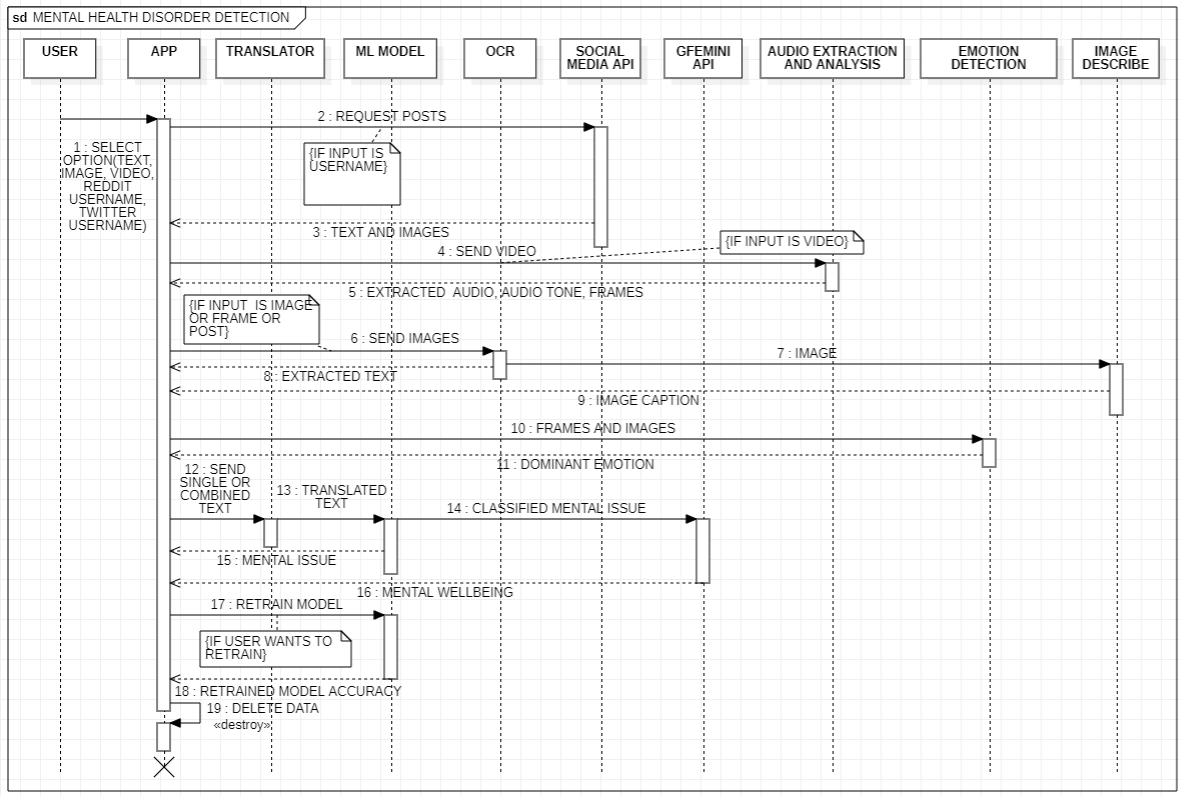
\includegraphics[width=1.0\textwidth]{Images/Sequence Diagram.png}  
    \caption{Application Sequence Diagram}
    \label{SequenceD}  % Label for referencing the figure
\end{figure}

\noindent
Below are some screenshots from the web application.

\pagebreak

\begin{figure}[h!]  
    \centering
    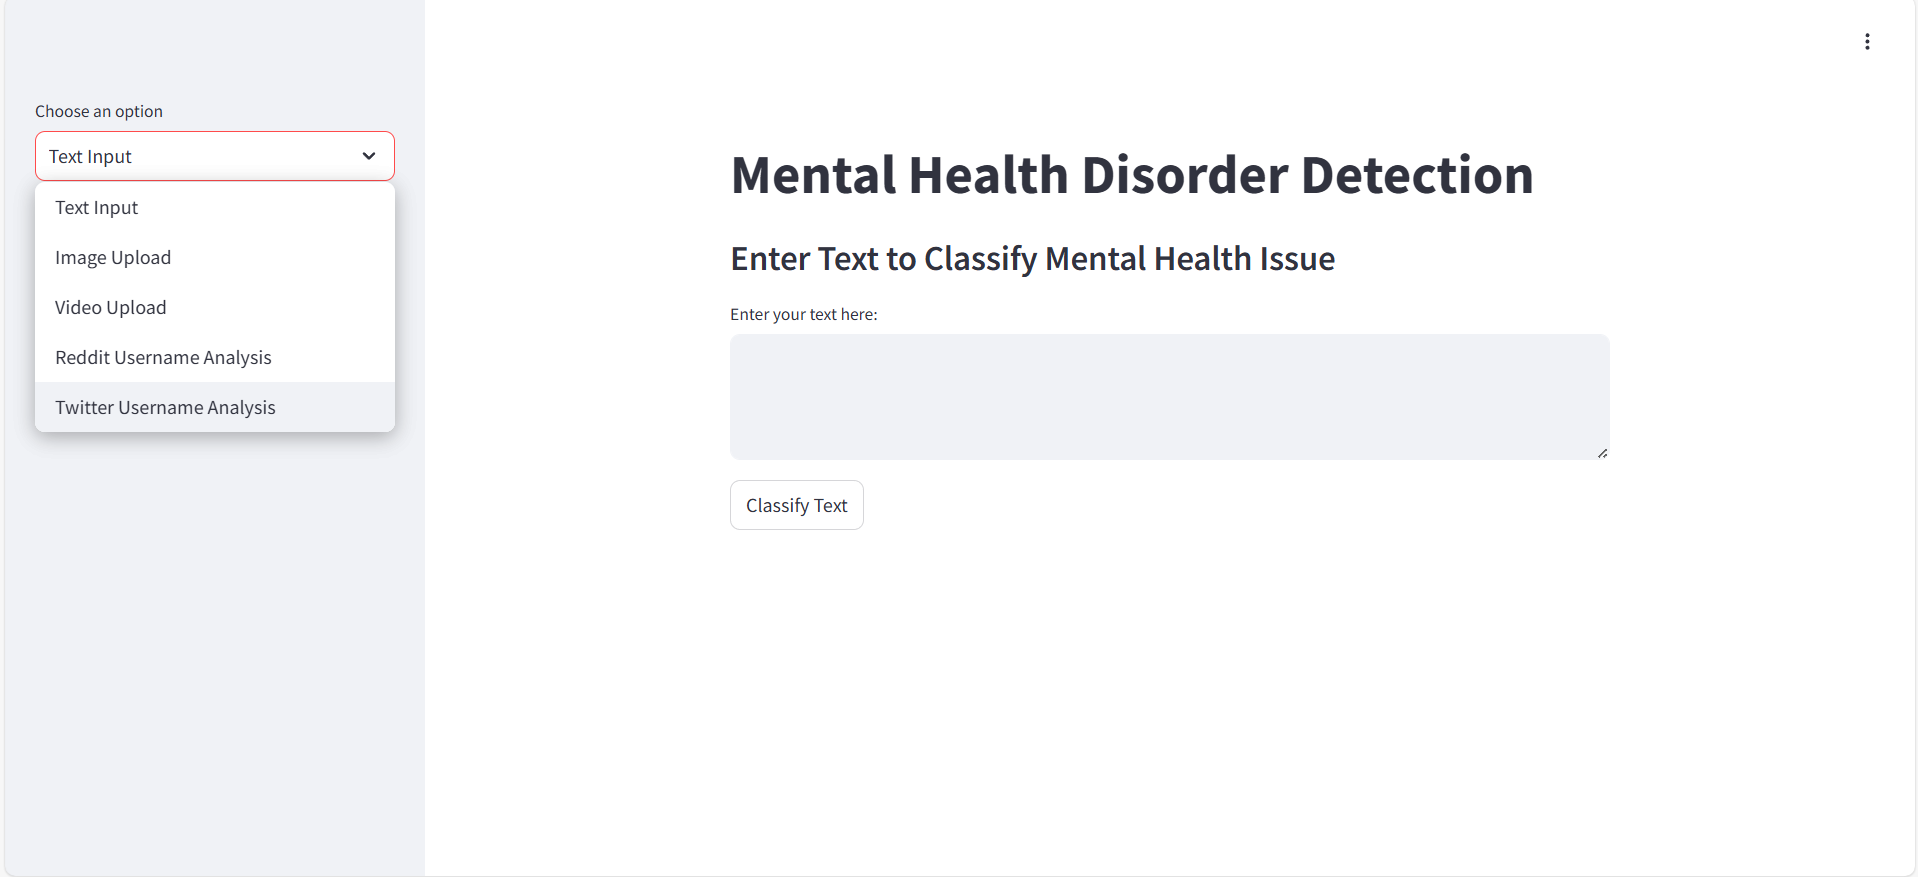
\includegraphics[width=1.0\textwidth]{App Images/01 Interface.png}  
    \caption{01 Website with all options}
    \label{01i}  % Label for referencing the figure
\end{figure}

\begin{figure}[h!]  
    \centering
    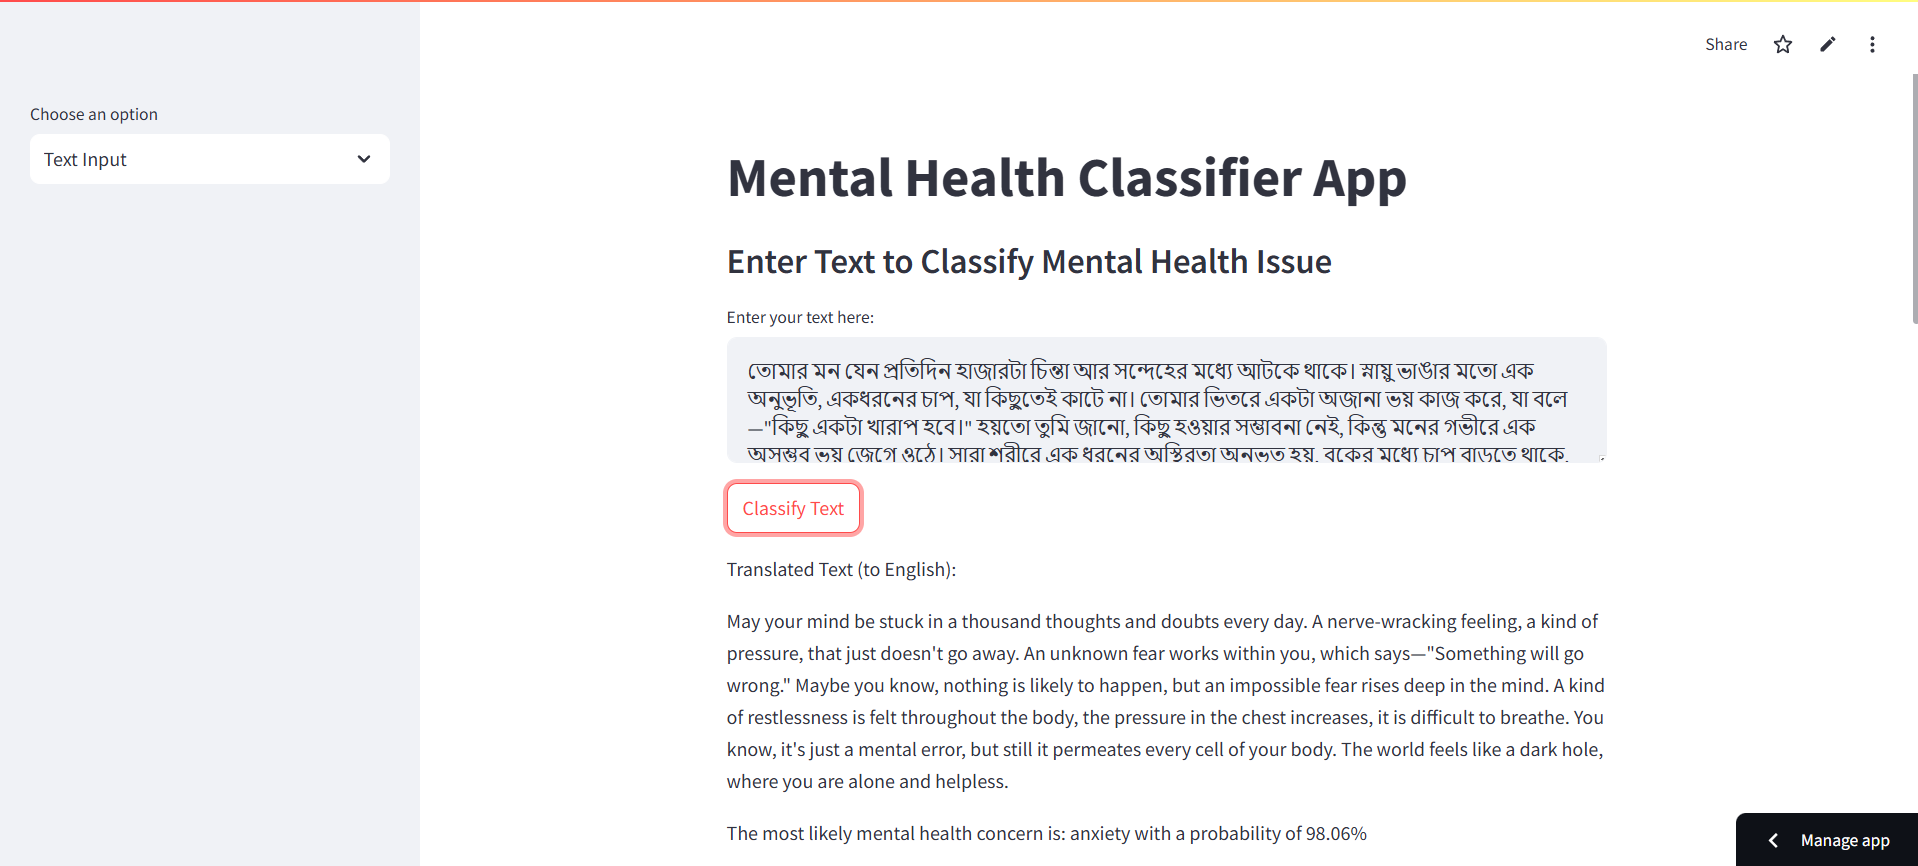
\includegraphics[width=1.0\textwidth]{App Images/02 Interface.png}  
    \caption{02 Entering Text for classification}
    \label{02i}  % Label for referencing the figure
\end{figure}

\begin{figure}[h!]  
    \centering
    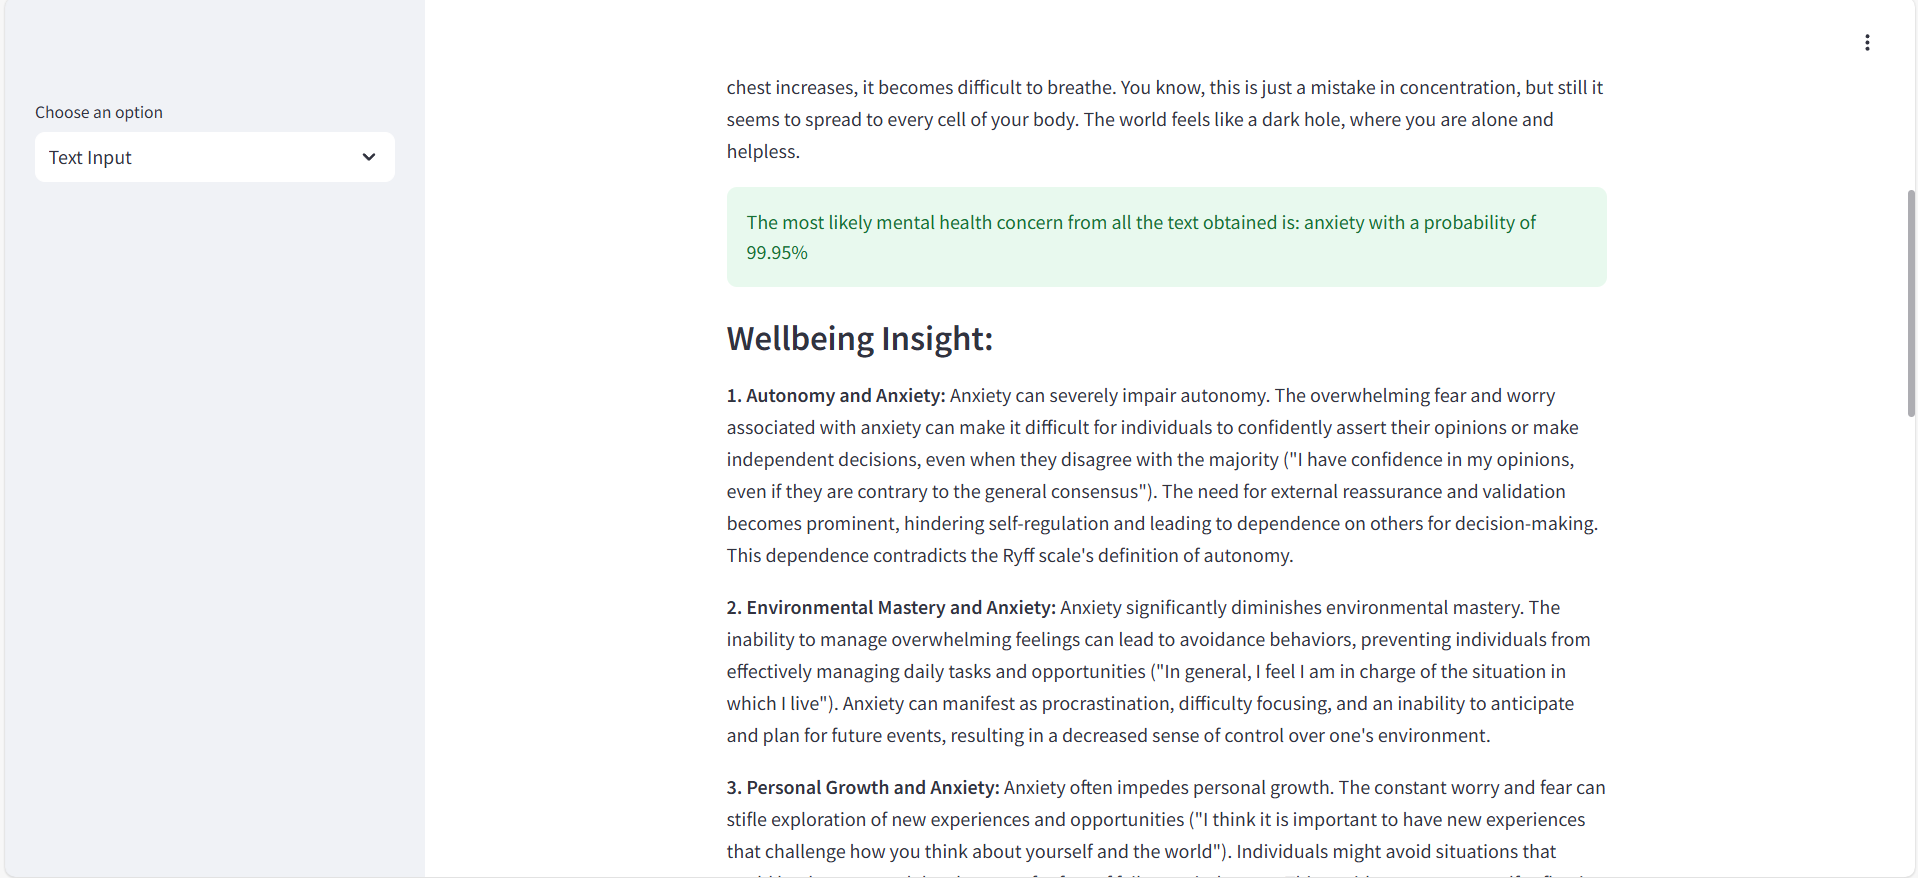
\includegraphics[width=1.0\textwidth]{App Images/03 Interface.png}  
    \caption{03 Text Classification Result}
    \label{03i}  % Label for referencing the figure
\end{figure}

\begin{figure}[h!]  
    \centering
    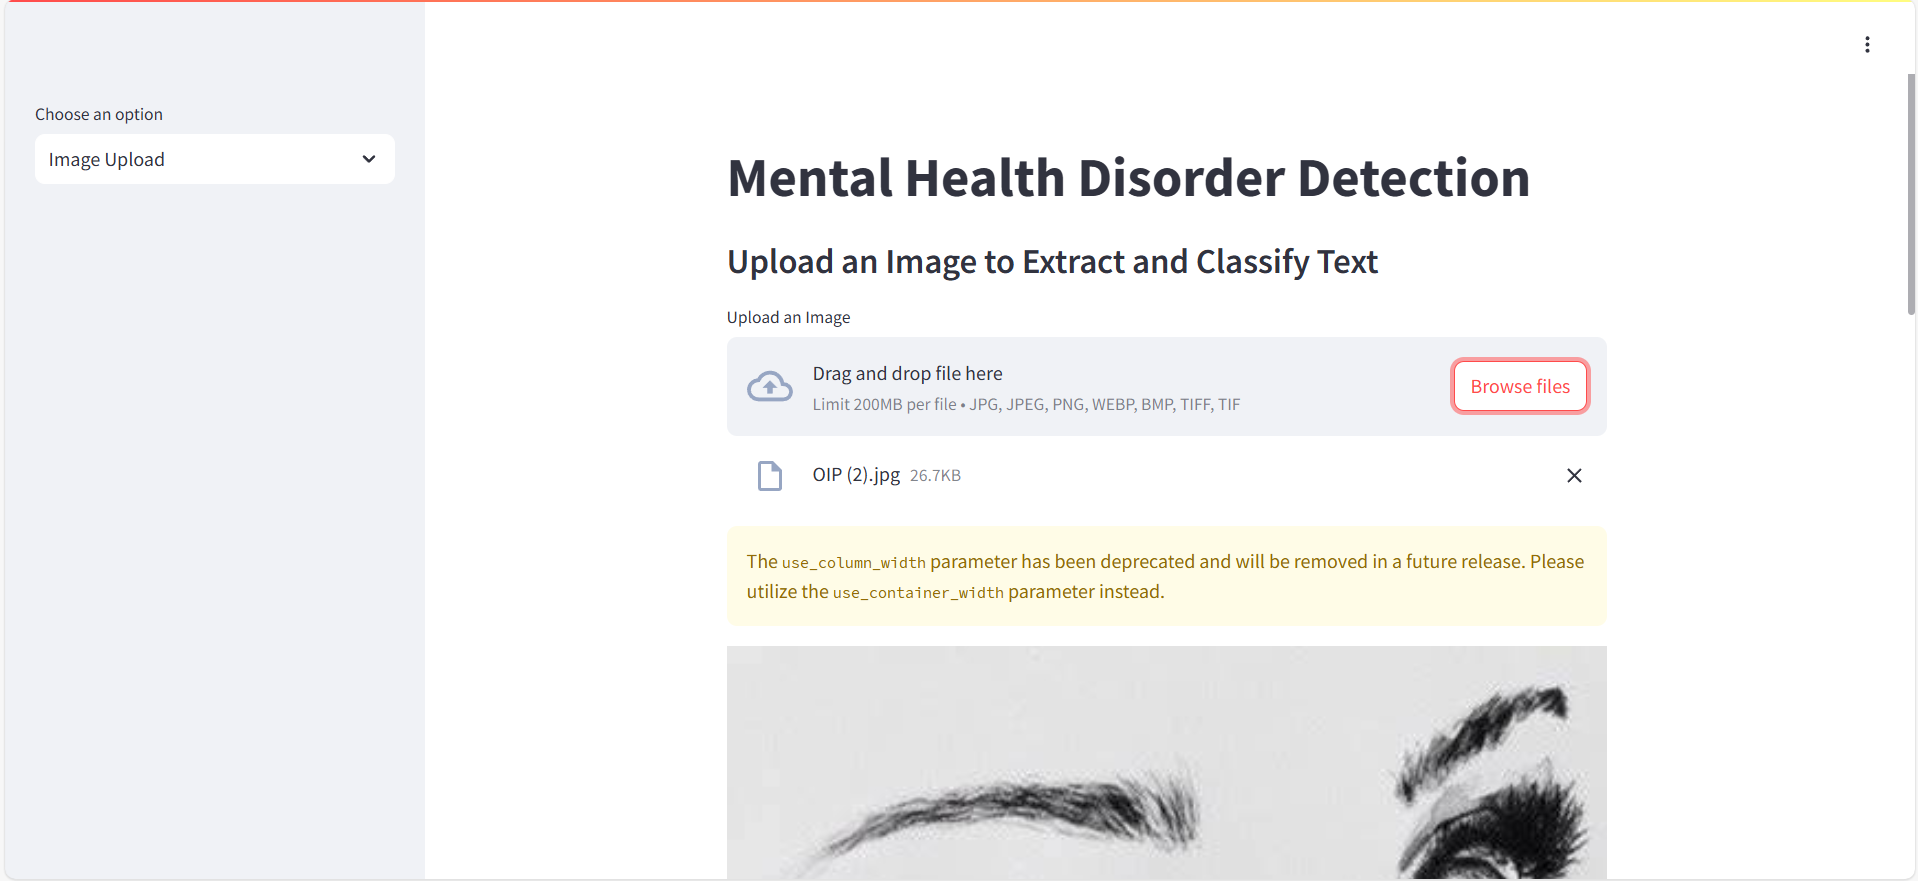
\includegraphics[width=1.0\textwidth]{App Images/04 Interface.png}  
    \caption{04 Image Classification}
    \label{04i}  % Label for referencing the figure
\end{figure}

\begin{figure}[h!]  
    \centering
    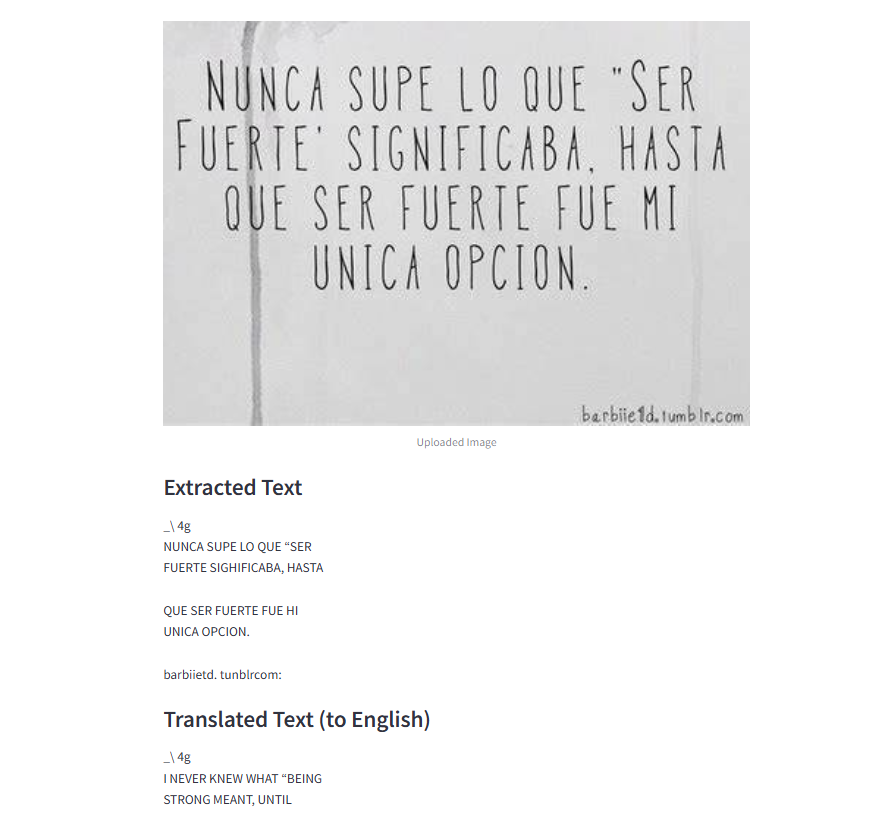
\includegraphics[width=1.0\textwidth]{App Images/05 Interface.png}  
    \caption{05 Extracted Text from Image}
    \label{05i}  % Label for referencing the figure
\end{figure}

\begin{figure}[h!]  
    \centering
    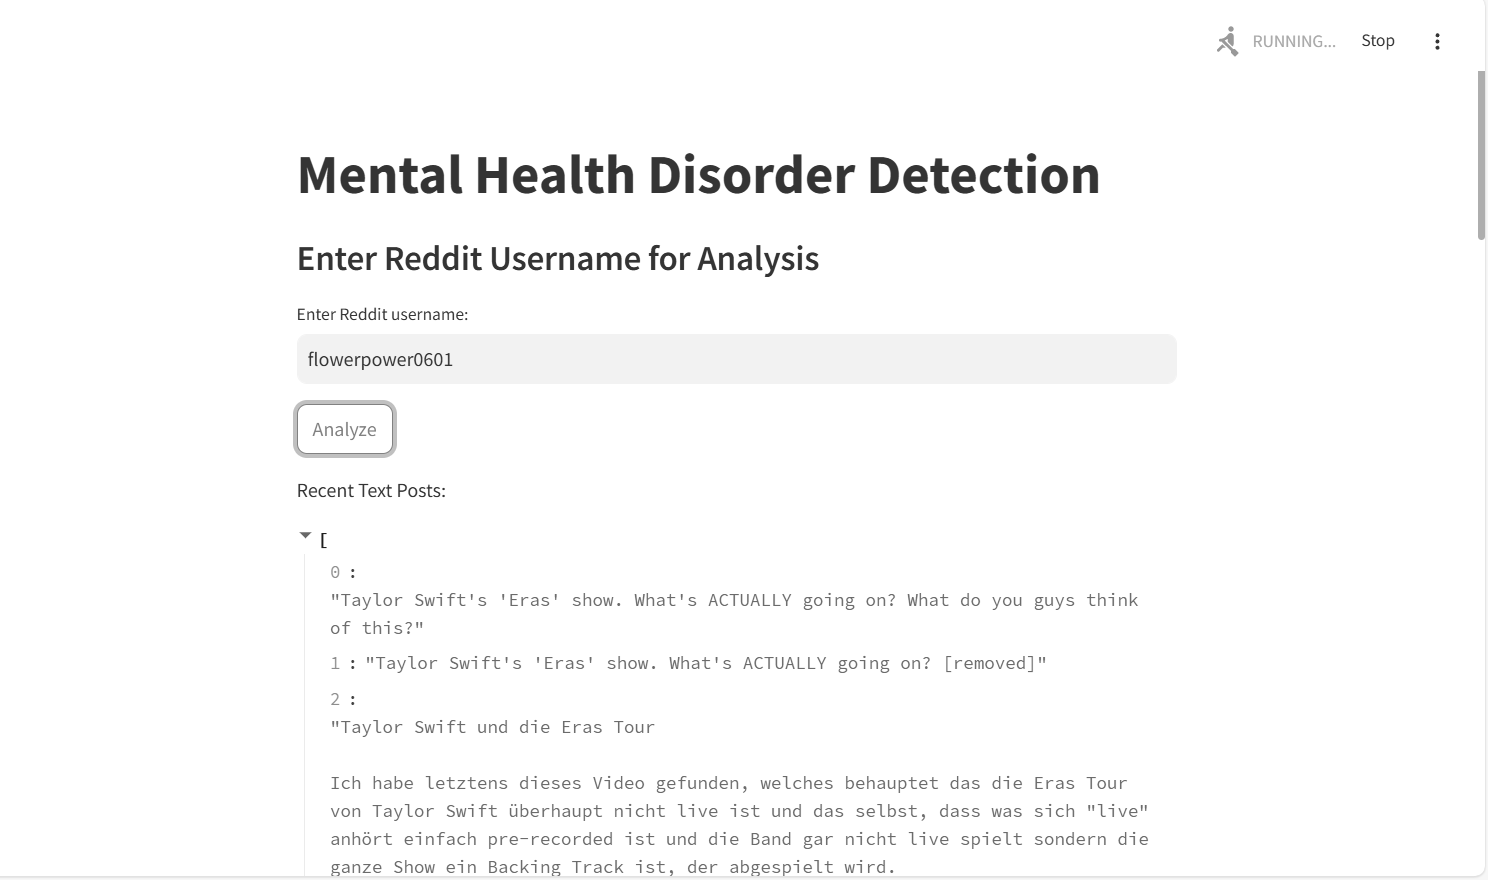
\includegraphics[width=1.0\textwidth]{App Images/06 Interface.png}  
    \caption{06 Image Classification Result}
    \label{06i}  % Label for referencing the figure
\end{figure}

\begin{figure}[h!]  
    \centering
    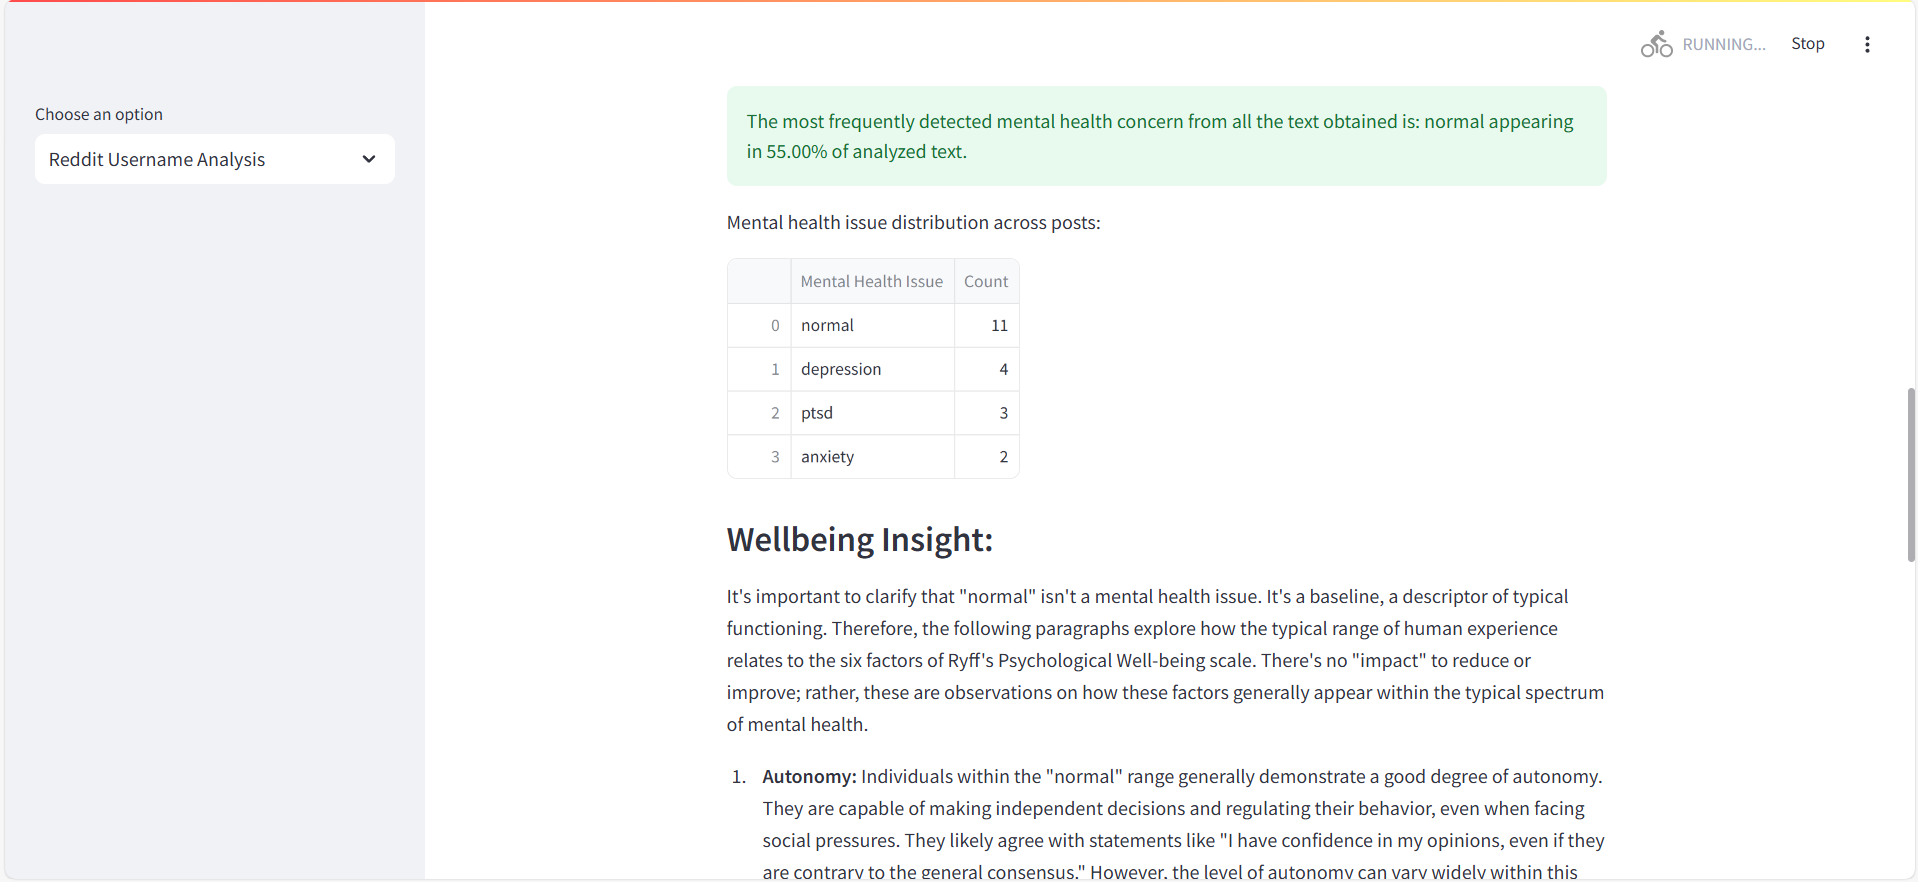
\includegraphics[width=0.9\textwidth]{App Images/07 Interface.png}  
    \caption{07 Reddit User Analysis}
    \label{07i}  % Label for referencing the figure
\end{figure}

\begin{figure}[h!]  
    \centering
    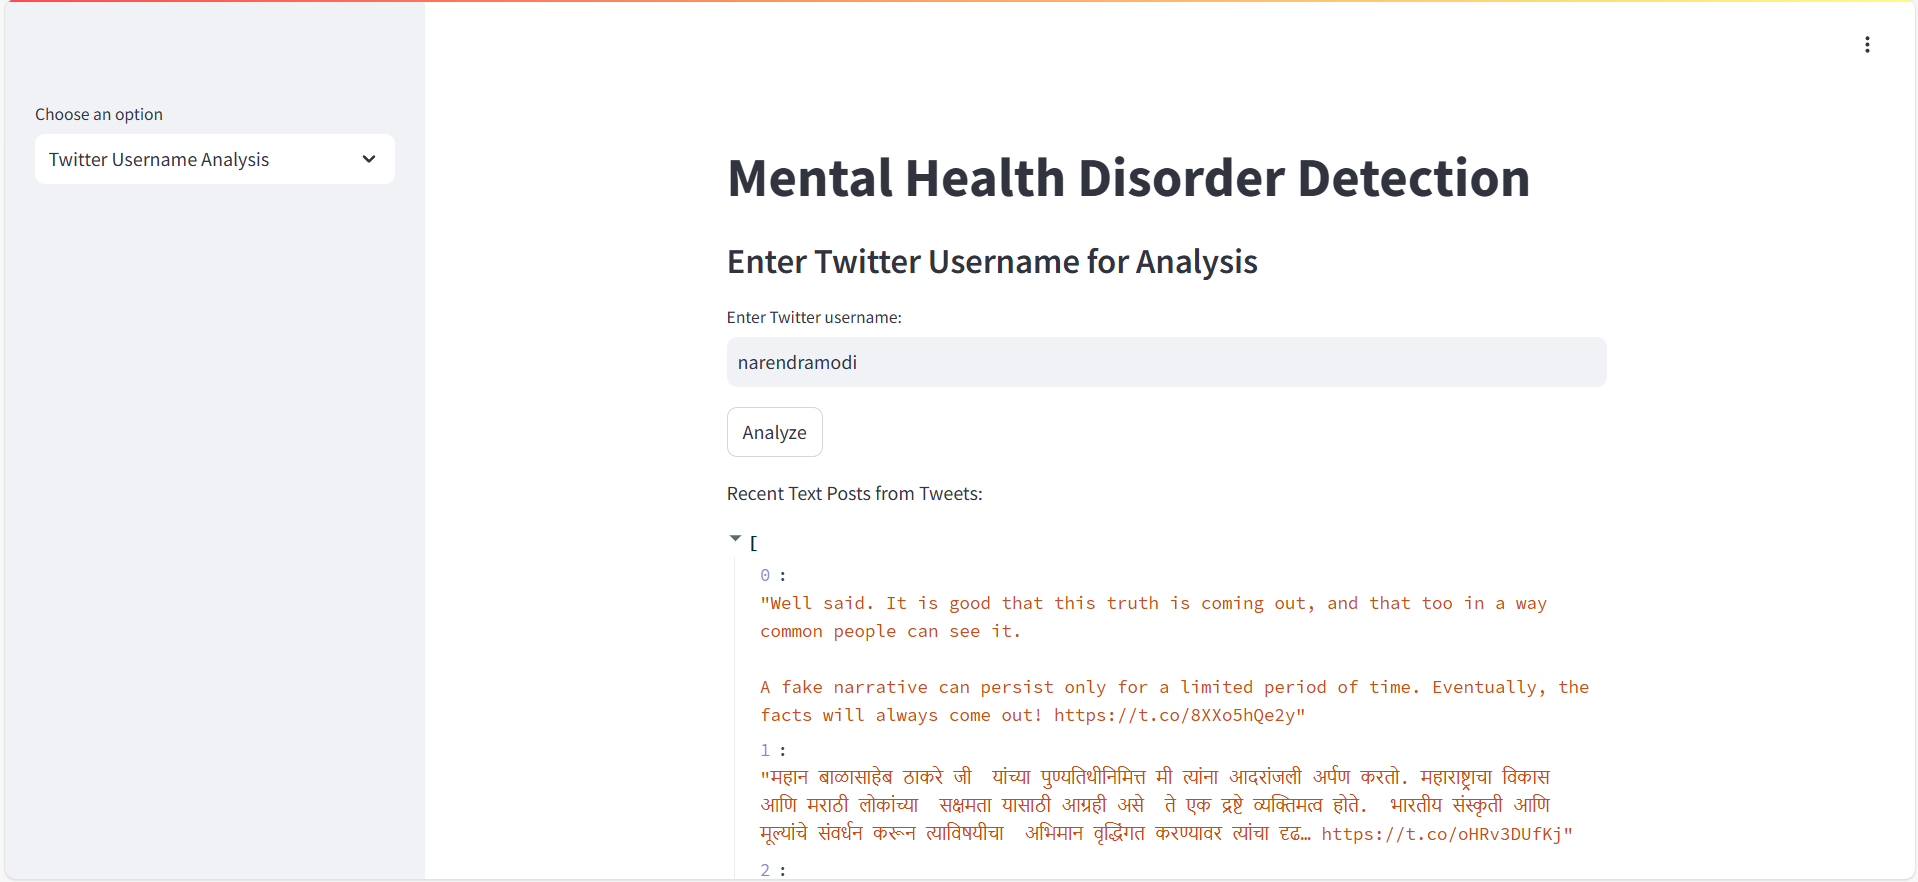
\includegraphics[width=0.9\textwidth]{App Images/08 Interface.png}  
    \caption{08 Posts from user profile}
    \label{08i}  % Label for referencing the figure
\end{figure}

\begin{figure}[h!]  
    \centering
    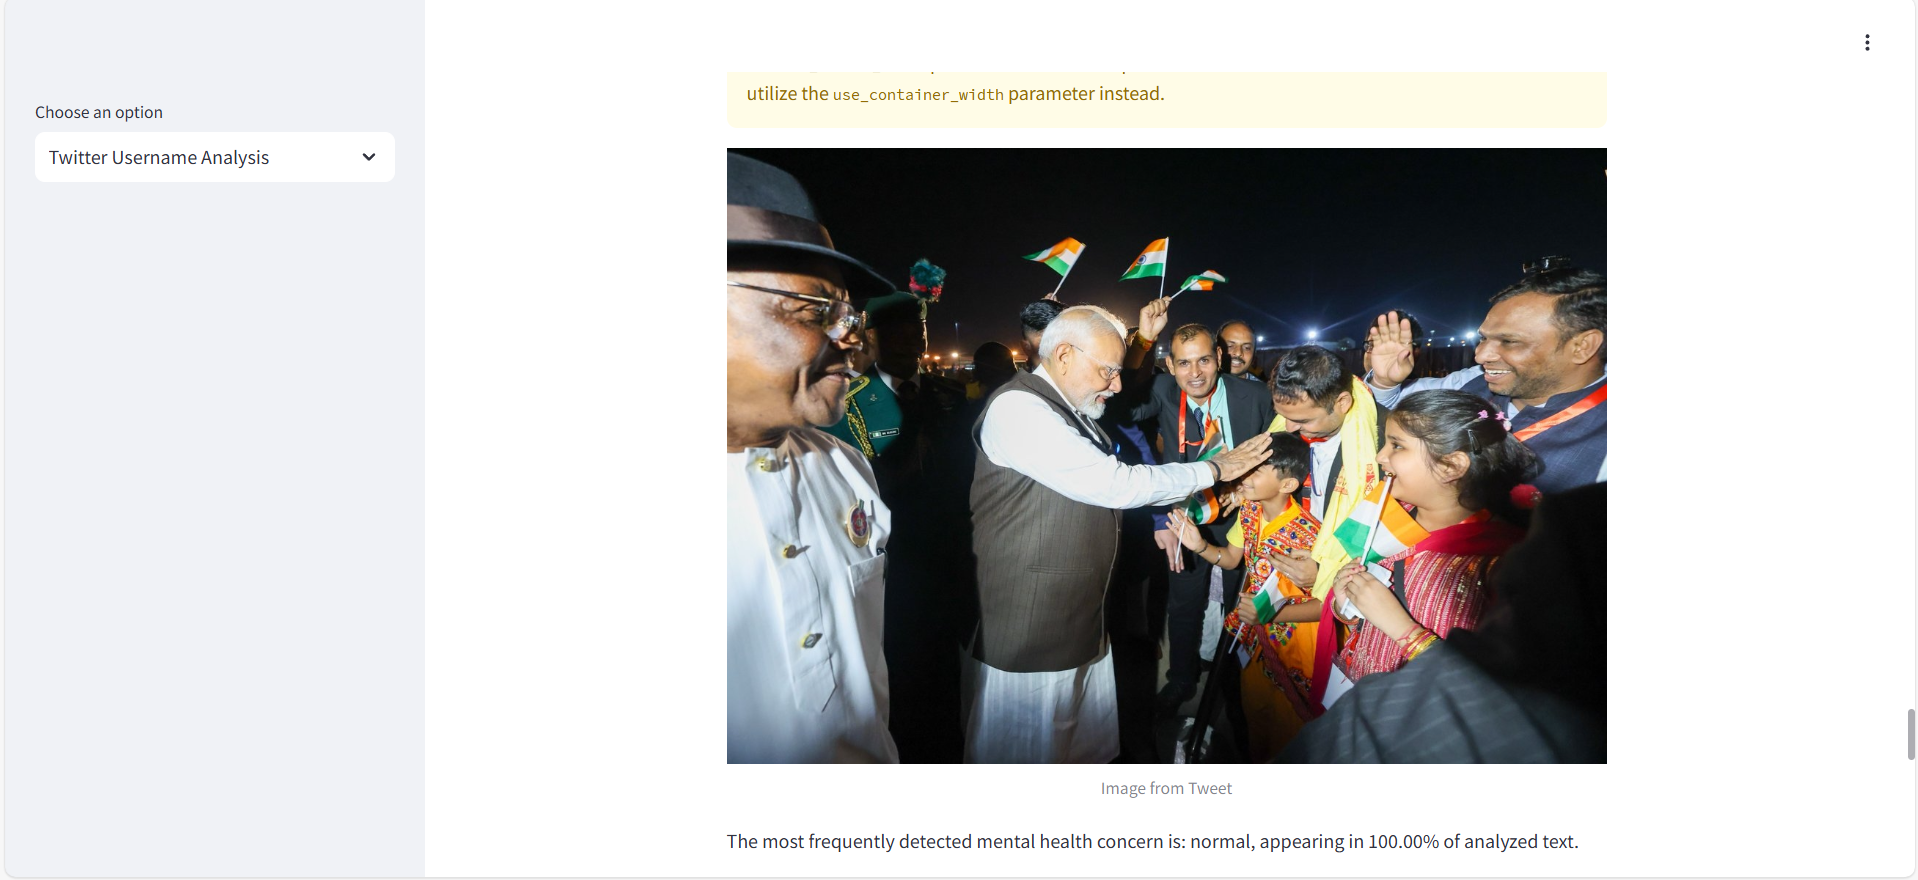
\includegraphics[width=1.0\textwidth]{App Images/09 Interface.png}  
    \caption{09 User profile Classification Result}
    \label{09i}  % Label for referencing the figure
\end{figure}




% ----------------------- Prototype ends -------------------


\begin{comment}

    \section*{APPENDIX B - Paper publications (optional) \label{sec:pubs}}
\addcontentsline{toc}{section}{APPENDIX B - Paper publications (optional)}
If any of your related paper(s) were published in a standard journal / presented in a recognized conference, mention the same including communication on your paper(s) acceptance / publishing note. You should also show appropriate documentation at the time of project viva.


\end{comment}

